%\vspace{10pt}
\section{Preliminaries}\label{sec:preliminary}

This section provides background of ReRAM and cross-point architecture,
and discusses the modeling of cross-point ReRAM array.

\vspace{-5pt}
\subsection{Background of ReRAM Technology}
%Table~\ref{table:compare} compares the properties of state-of-art
%non-volatile memory technologies. ReRAM and STT-RAM are better than PCM or
%FeRAM due to their faster access time and high endurance. Although STT-RAM
%has better read/write delay characteristics, the difference in cell
%resistance between ON and OFF states is higher in ReRAM. Further more,
%ReRAM has the best memory density. Hence, ReRAM is a leading candidate for
%next generation storage.
%%
%%shows the fastest read/write latency among all non-volatile memory technologies, the structure of the memory cell is complex and it has a large cell size. On the other hand, the ReRAM has a very simple cell structure and can be implemented with an area efficient cross-point structure, which can work without any access devices. This simple structure provides the possibility of high density integration and 3-D stacking /* DOES THAT MEAN STT-MRAM IS NOT 3D FRIENDLY? ALSO, HOW SIMPLE STRUCTURE & 3D ARE RELATED? */ of ReRAM based memory arrays. Besides, the ReRAM has much higher ON-OFF resistance ratio than STT-RAM. With all of these advantages, the ReRAM based memory is considered as a highly competitive technology compared to all other emerging non-volatile memory technologies.
%
%\begin{table}[!tb]
%  \centering
%  \scriptsize
%    \scriptsize
%  \caption{Comparison of Emerging Non-Volatile Memory Technologies}\label{table:compare}
%  \vspace{-0pt}
%%  \begin{tabular}{|cccccp{3.5cm}|}
%  \begin{tabular}{|c|cccc|}
%    \hline
%    % after \\: \hline or \cline{col1-col2} \cline{col3-col4} ...
%    \textbf{Metric} & \textbf{STT-RAM} & \textbf{PCM}    & \textbf{FeRAM} & \textbf{ReRAM}
%    \\\hline
%    \textbf{Cell Size($F^2$)} & $6-20$ & $4-8$ & $15$ & $4$\\\hline
%    \textbf{Read Latency(ns)} &  1-10 & 20-50 & 20-80 & 5-50\\\hline
%    \textbf{Write Latency(ns)} & 2-20& 150& 100& 5-50\\\hline
%    \textbf{Endurance} &  $10^{15}$ & $10^8$ & $10^{12}$ & $10^{8-10}$\\\hline
%  \end{tabular}
%  \vspace{-5pt}
%\end{table}

%Different from the traditional memory technologies, which use the electron stored in the cell to represent the information, the non-volatile memory use the the phase/state/resistance of the memory cell itself to store the data. Therefore, the nonvolatile memory can retain the stored information without pow supply. This kind of non-volatility make it a potential candidate as the alternative memory technology to replace the DRAM even SRAM technologies.

As implied by its name, a ReRAM cell uses its resistance to represent the
stored information. A ReRAM cell is built on a Metal-Insulator-Metal(MIM)
structure and can be switched between a high resistance state (HRS) and a
low resistance state (LRS) by applying an external voltage across the
cell. The resistance switching behaviors have been observed in many MIM
nanodevices with different metal oxide materials. For example, a
particular $TiO_2$ based MIM structure ReRAM, named `memristor', was
developed by HP Labs in 2008~\cite{memristor:missing}. The proposed
memristor-based ReRAM is considered as the first experimental realization
and a theoretical model of the fourth fundamental circuit element, which
is predicted by Chua~\cite{memristor:chua} about 40 years ago. It has been
reported that the memristor-based ReRAM has very small cell size with an
access time of less than 50ns~\cite{memristor:switch}.
%/*(WHAT IS THE SIGNIFICANCE OF 50x50nm2 SIZE? AT WHAT TECHNOLOGY? */
Another $H_fO_2$-based bipolar ReRAM prototype was fabricated by ITRI with
an access time as low as 7.2ns~\cite{ReRAM_ISSCC2011_Sheu}.
%The memristor based ReRAM built by HP Labs has a two-terminal, two-layer structure. The top and the bottom electrodes are nanowires made by Pt. Two layers of titanium dioxide are sandwiched between these two electrodes in
%a crossbar architecture. By applying an external voltage across the cell, the memristor can switch between two stable states: ON
%state with low resistance and OFF state with high resistance. A
%positive voltage above a specific threshold will switch the device
%into the OFF state (SET operation) and a negative voltage of the
%same magnitude toggles it to its ON state (RESET operation). T

Although there are several variants of ReRAM cells, all of them can be
classified into two broad categories: unipolar ReRAM and bipolar ReRAM. In
a unipolar cell, the resistance switching behaviors do not depend on the
polarity of the voltage input across the cell and are only related to magnitude
and duration of the voltage input. On the other hand, in a bipolar cell,
the voltage polarity for ON-to-OFF switching (RESET operation) is
different from OFF-to-ON switching (SET operation).
%Unipolar ReRAM can be easily stacked on top of a diode to build a one diode one resistor (1D1R) ReRAM~\cite{memristor:1D1R}. SINCE BIPOLAR RERAM CAN ALSO USE ACCESS DEVICE, WHAT IS THE VALUE OF THIS LINE?
%However, since SET and RESET operations have different latencies, the performance of unipolar ReRAM is limited by the longer voltage pulse.
The need of different pulse widths for SET and RESET in unipolar ReRAM
means that its write latency is determined by the longest pulse. Moreover,
the control of SET, RESET, and read operations without any disturbance is
another crucial design challenge, especially in high speed ReRAM design.
For these reasons, most high performance ReRAM studies are dominated by
bipolar
ReRAM~\cite{ReRAM_IEDM2010_Kim,crossbar_Panasonic,ReRAM_ISSCC2011_Sheu,ReRAM_ISSCC2011_Otsuka}.
%However, the bipolar ReRAM also has its inherent problems as they lack access device in cells. IN THE NEXT PARA BEGINNING, YOU SAY WE CAN USE MOS ACCESS DEVICE. SO THIS SHOULDN'T BE AN INHERENT PROBLEM.
In this study, we perform a detailed analysis of the design challenges of
bipolar ReRAM cross-point arrays.

\vspace{-5pt}
\subsection{Cross-Point Architecture}
There are two possible memory structures for a bipolar ReRAM array
implementation: the traditional MOSFET-accessed structure and the
cross-point structure. In the MOSFET-accessed memory array, a MOSFET is
used as an access device for each memory cell. As the size of a MOSFET
access device is typically much larger than the size of a ReRAM cell, the
total area of memory array is primarily dominated by MOSFETs rather than
ReRAM cells. Also, in order to provide enough driven current, larger than
minimum-sized transistor should be used for write operations. Hence,
ReRAM's area advantage gets lost because of the access devices.
%The ReRAM's advantage of ultra small cell size will be offset by the access device.
Fortunately, the access device can be eliminated due to the large
current-voltage (I-V) nonlinearity of some ReRAM
devices~~\cite{memristor:switch,memristor:Unity}. The I-V characteristic
demonstrated in these fabricated devices shows that the resistance of
ReRAM significantly increases as the voltage applied on it decreases. Such
observation basically indicates effective cut off of the leakage current
from the unselected cells in the sneak paths. Therefore, the
area-efficient cross-point ReRAM memory array is enabled by the intrinsic
property of the device~\cite{memristor:Cong}. A schematic view of a
typical cross-point memory array is shown in Figure~\ref{fig:array}(a). As
shown, ReRAM cells are sandwiched between wordlines and bitlines (top
electrodes and bottom electrodes). Figure~\ref{fig:array}(b) shows a top
view of the array, which indicates that each ReRAM cell occupies an area
of $4F^2$, the theoretical lower limit for a single layer single level
memory cell. In addition, this memory density can be further improved by
using a multi-layer multi-level cross-point ReRAM
array~\cite{crossbar_unity}~\cite{memristor:IEDM08_3D}.
%Besides, as aforementioned, the good stackability and the high resistance ratio provide the capability of building a multi-layer multi-level cross-point ReRAM array, which can further increase the area efficiency~\cite{ReRAM_ISSCC2011_Sheu}~\cite{memristor:IEDM08_3D}.

\begin{figure}
\centering
  % Requires \usepackage{graphicx}
  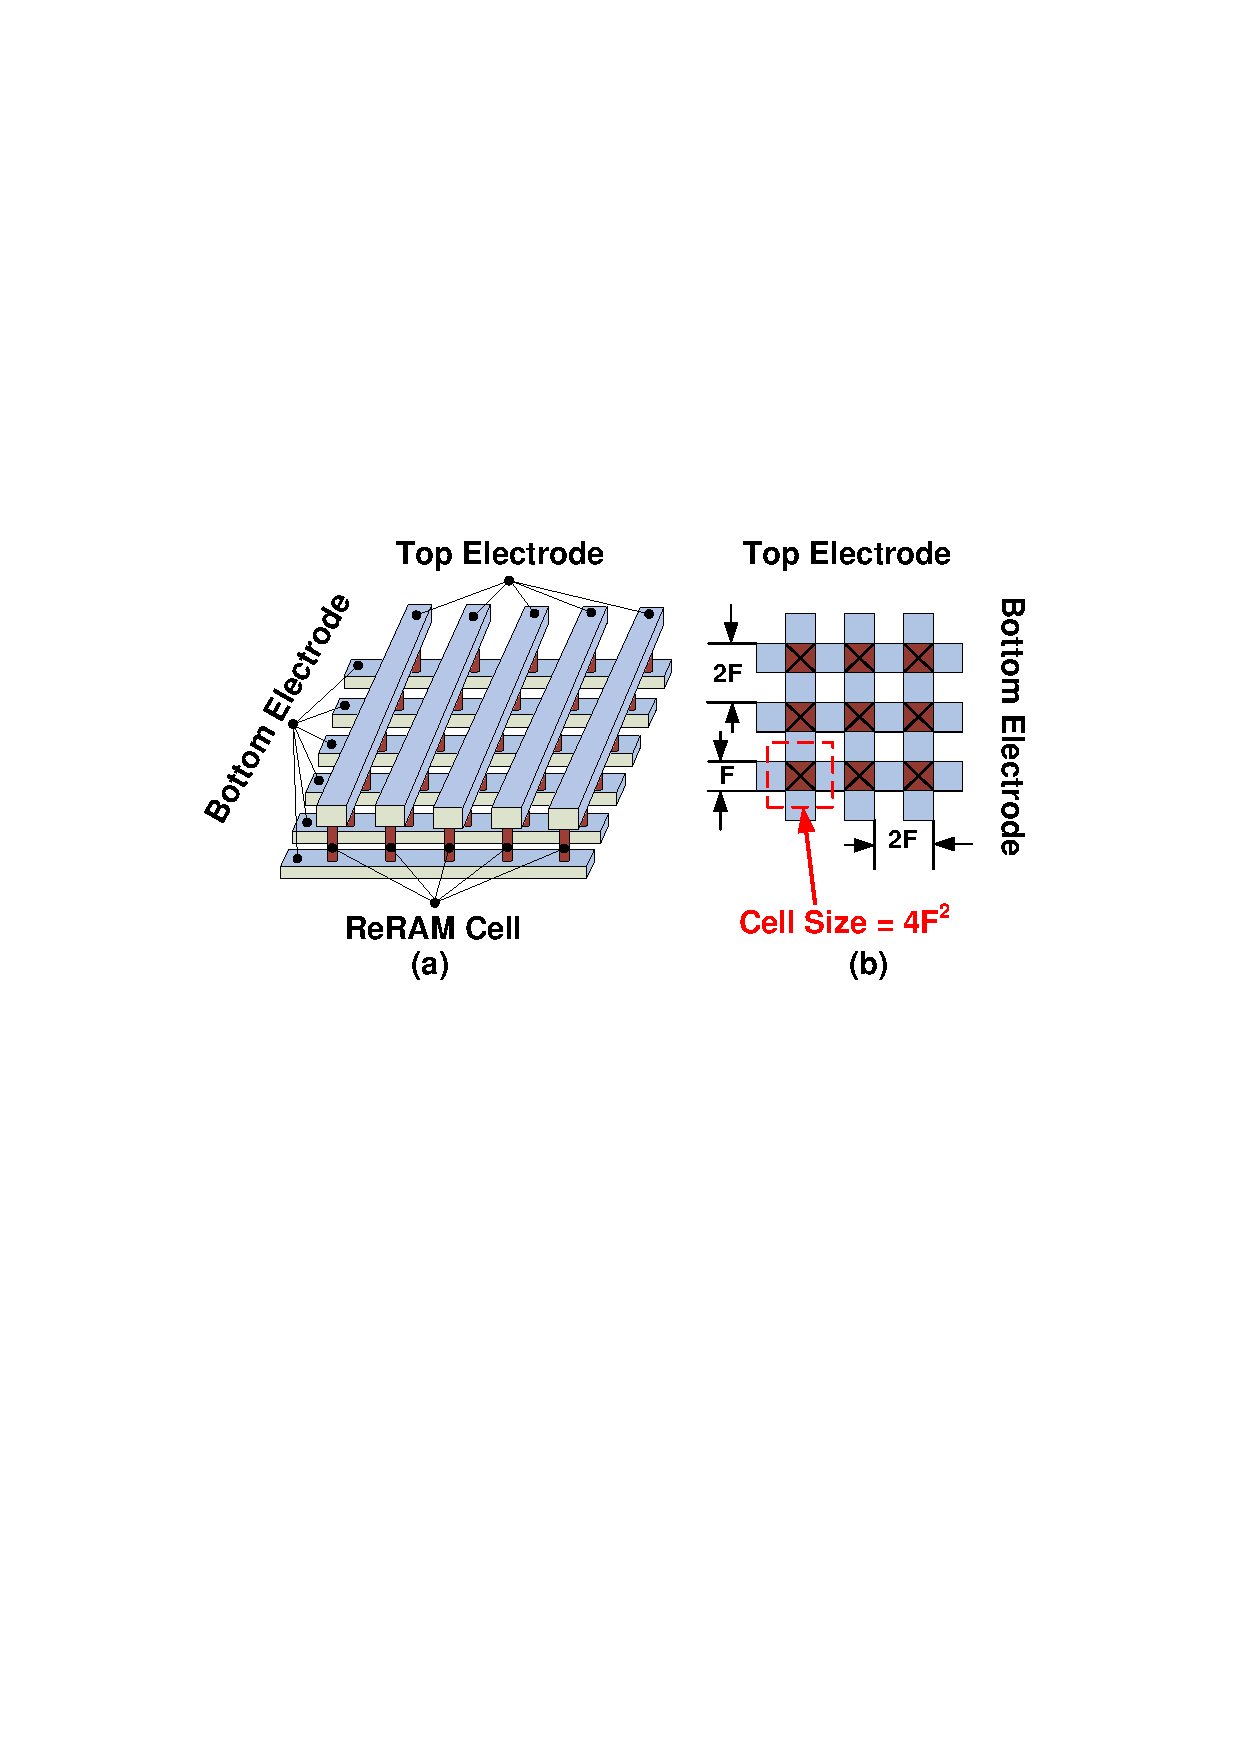
\includegraphics[width=0.45\textwidth]{./figures/crossbar_array2.pdf}\\\vspace{-10pt}
  \caption{A schematic view of a typical cross-point array. (a) The perspective of the cross-point array.
  (b) The top view of the array, from which we can clearly see that the size of each cell is $4F^2$. }\label{fig:array}
\vspace{-12pt}
\end{figure}

There are several write/read schemes for cross-point ReRAM arrays. For
example, the write operation can write either a single-bit per access or
several bits attached to the same wordline at the same time. Although the second
scheme has higher bandwidth, it requires a two-step write operation to
prevent unintentional writing~\cite{memristor:Cong}, which significantly
increases the write latency.
%Therefore, the write latency for the multi bit write operation is much larger than the one bit operation.
Furthermore, while writing to a cross-point array, the unselected wordlines
and bitlines can be either left floating or half-biased. In contrast, while reading
a cell, the selected wordline should be biased with a read
voltage and all the other wordlines and bitlines in the array are shunted
to ground. The current in each bitline is then sensed and compared to a
reference current to determine the cell content. However, due to the sneak
current existing in the cross-point array, the current in bitlines also
varies depending upon the data patterns of unselected cells.
%is impacted significantly by the data pattern of the unselected cells in the array.
This read disturbance restricts the size of a cross-point array, since
sneak current increases as the number of cells attached to wordlines and
bitlines increases, which makes it difficult to sense the current
difference of the selected cell at HRS and LRS. Besides, the existence of
the voltage drop along the nanowires also limits the length of wordlines
and bitlines. Therefore, a cross-point array should be sized carefully to
meet the requirements of the read/write reliability.
%Therefore, a cross-point array should be sized carefully such that the current difference of the selected cell at HRS and LRS is large enough for reliable sensing.
In addition to all of these write/read schemes, different cell parameters
will also impact the reliability, energy consumption, bandwidth, and area
efficiency of the cross-point ReRAM array. In this case, it is not
straightforward for a designer to figure out how to design a workable
memory array with the minimum energy consumption and area overheads. Thus,
the following sections will propose a worst-case oriented methodology to
help designers make decisions early in the design flow.

%Depending upon the read/write scheme, the size of the array can vary significantly. In this work, we propose a methodology to find the minimum array size that meets specific energy and area constraints based on the worst-case state of the array. This will help designers find an optimal memory organization early in the design flow. %t read/write schemes as well as array sizes can be chosen for the cross-point array, it is not straightforward to figure out how to design a workable memory array with the minimum energy consumption and area overheads. Thus, following sections will proposed a worst-case oriented methodology to help designer make the decision early in the design flow.


%\subsection{Limitations of Cross-Point Architecture}
%\subsection{Related Work and Motivations}
%Although the cross-point structure can provide the fabricate simplicity and area efficiency, it also incur lots of design challenges. Many of the design challenges, such as the array size, resistance ratio as well as the data pattern have been presented and analyzed by previous researches. However, all of these researches focus on the cross point array itself and do not take into account the area or energy overhead of the peripheral circuit. Besides, a comprehensive study on different write/read schemes is also lacking. In this
%
%
%One of the well known design challenge of cross-point is the sneak path existed in the memory array, which will lead a read failure during the read operation and bring in extra energy consumption. Besides, there are also several design options can be chose during the system design. Following shows an example, which shows part of the design challenges of the cross-point structure motivates the work in this paper.
%\begin{enumerate}
%  \item \textbf{Example of the Design Challenges of Cross-Point Structure.}\\
%  In order to
%
%\begin{figure}
%\centering
%  % Requires \usepackage{graphicx}
%  \includegraphics[width=0.4\textwidth]{./figures/example1_large.pdf}\\
%  \caption{Case 1: Voltage Drop Along the Word Line during Write Operation.}\label{fig:exampl1}
%\end{figure}
%
%  \item \textbf{Read Margin Disturbance}\\
%  123
%  \item \textbf{Energy Waste Due to Sneak Pass}\\
%  123
%\end{enumerate}
%
%~\cite{crossbar_NANO08_Nauenheim}~\cite{memristor:analog}~\cite{moore}
%
\vspace{-5pt}
\subsection{Modeling of the Cross-Point Memory}\label{sec:model}

%\subsection{Basic model of Cross-Point Memory}
The basic circuit model of an $M$ by $N$ cross-point ReRAM array is shown
in Figure~\ref{fig:modeling}. This model is built upon Kirchhoff's Current
Law (KCL) and its validity can be guaranteed by deductions from basic
circuit theory. The horizontal lines are wordlines and the vertical lines
represent bitlines. The ReRAM cells are located at each wordline and
bitline cross-point. A detailed cross-point structure is also shown in
Figure~\ref{fig:modeling}(b). The resistance of the ReRAM cell at the
cross-point of $i^{th}$ wordline and $j^{th}$ bitline is represented by
$R_{i,j}$. We assume the resistance of the wire connecting two
cross-points to be $R_{line}$. The input resistance of each wordline or
bitline driver is $R_v$ and the resistance of a sense amplifier is $R_s$.
In order to set up the KCL equations, the voltage at each cross-point is
indicated as $V_{i,j}$ for the wordline layer and $V'_{i,j}$ for the
bitline layer. In addition, the input voltage for the $i^{th}$ wordline is
$V_{Wi}$ and for the $i^{th}$ bitline is $V_{Bi}$. In the case that a
wordline is driven from both sides, the voltage at the other end of the
$i^{th}$ wordline is represented as $V'_{Wi}$.

%Finally, the voltage at the sense amplifier is $V'_{Bi}$ during the read operation.
%YOU MIGHT WANT TO CHANGE THE ABOVE PARA INTO A TABLE

\begin{figure}%[!hb]
\centering
  % Requires \usepackage{graphicx}
  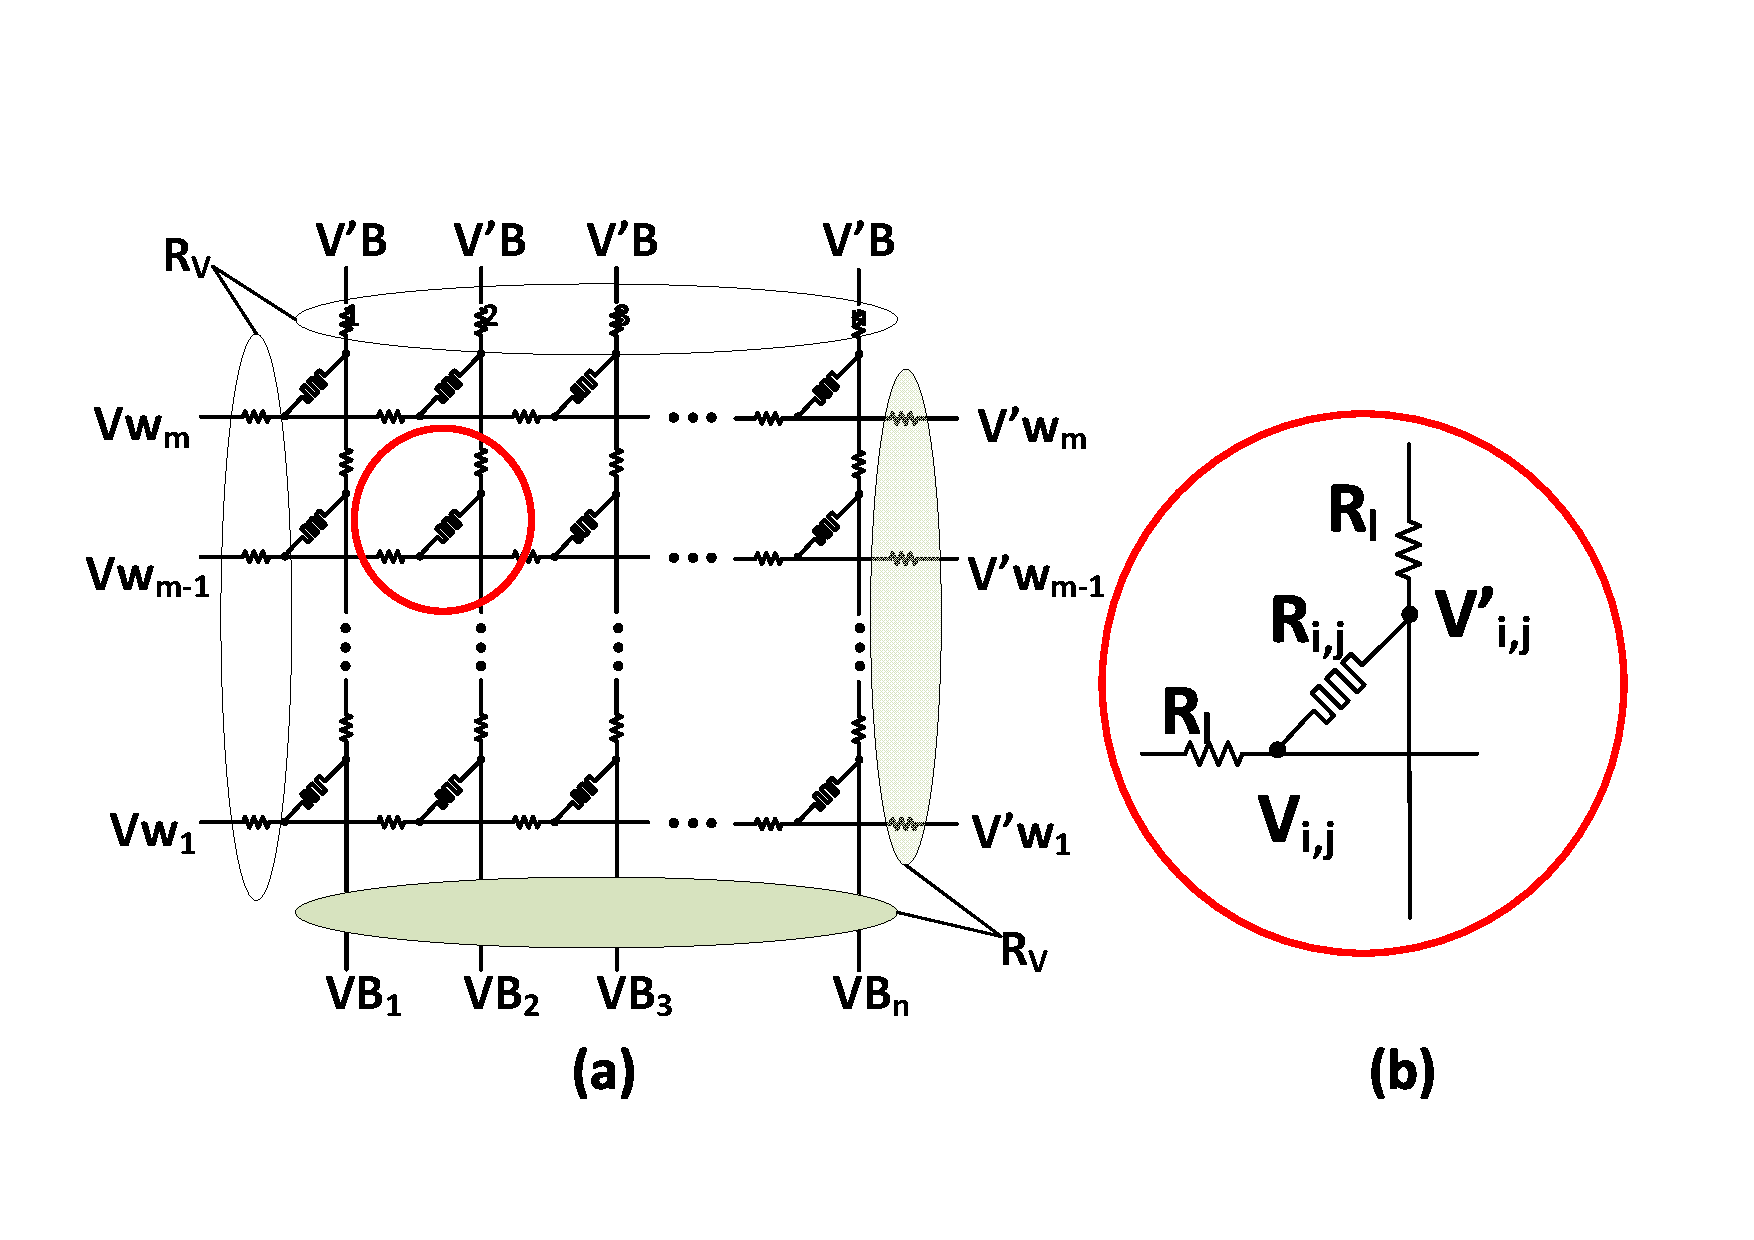
\includegraphics[width=0.45\textwidth]{./figures/model_f.pdf}\\
  \vspace{-8pt}
  \caption{The circuit model of the cross-point array.}\label{fig:modeling}
  \vspace{-4pt}
\end{figure}

%\subsection{Mathematical Model of a Cross-Point Array}
Based on this model, the current equations for each cross-point can be
obtained. All of the cross-points have similar structure with no more than
three current branches, and therefore it is very easy to set up the KCL
equations for each cross-point. Since the cross-points at the edges of the
array have different write/read conditions, the KCL equations of these
cross-point should be adjusted according to each write/read scheme.All of
the KCL equations can be considered as a system of linear equations, which
has the following form of {$ A\cdot~V~=~C $}, where $A$ is a
${2mn\times{2mn}}$ coefficient matrix and $C$ is a ${2mn\times{1}}$
vector, containing the constant terms of these equations. Thus, with
parameters such as the resistance of ReRAM cells, the resistance of
interconnect wires, program voltages, and write/read schemes, voltages at
various cross points can be obtained by solving the system of linear
equations. With detailed voltage values, $V_{2mn{\times}1}$, we can
analyze the array at a fine granularity. These values are also critical to
evaluate the reliability, energy consumption, driven current density, and
area overheads of a cross-point array.

To validate the analytical model, we compare the results with
HSPICE~\cite{HSPICE} simulations using a resistor model in cross-point
memory arrays. The results of eight cross-point arrays with different
array sizes and specific data patterns are shown in
Figure~\ref{fig:validation}, which shows that the voltage drop on the
selected cell derived from our analytical model are consistent with the
HSPICE simulation results.
\begin{figure}%[!t]
\centering\label{fig:SPICE}
  % Requires \usepackage{graphicx}
  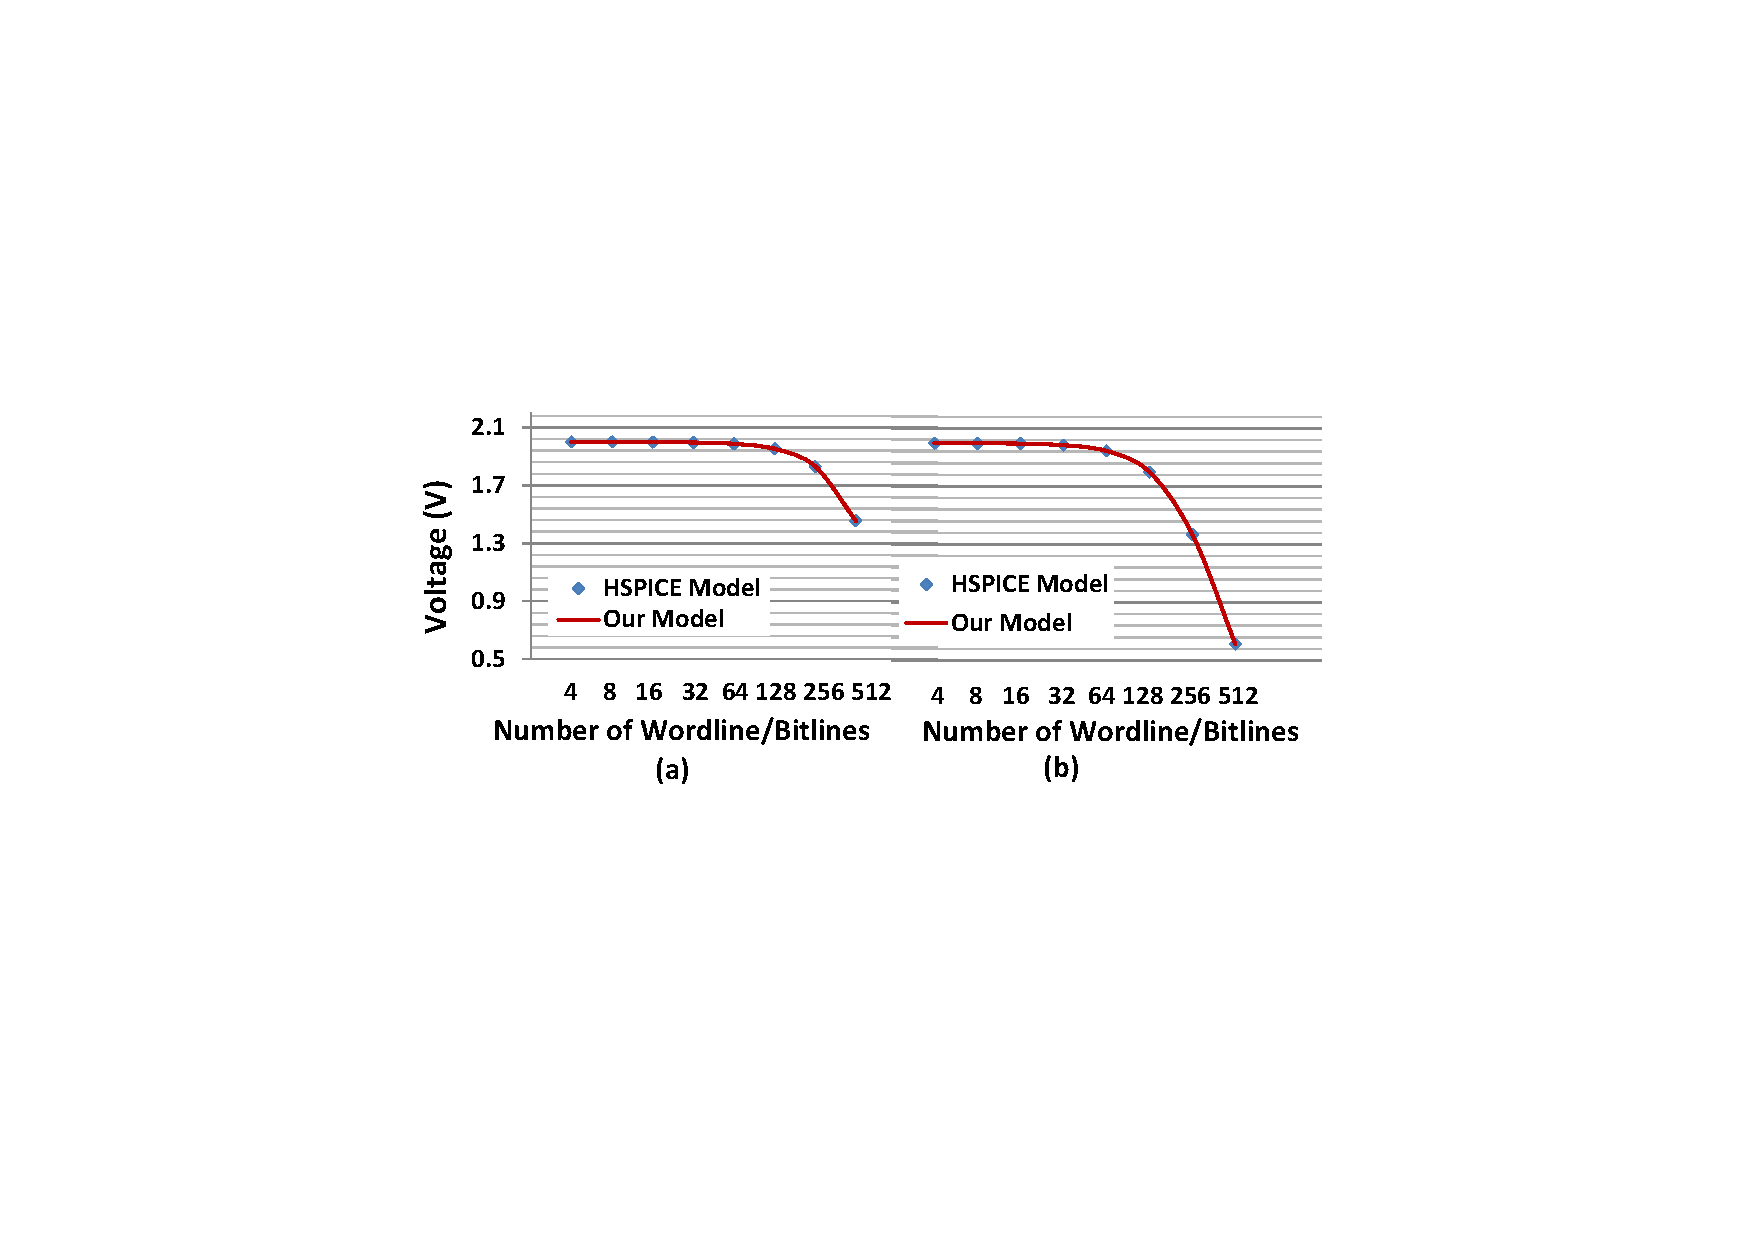
\includegraphics[width=0.5\textwidth]{./figures/SPICE1.pdf}\\
  \caption{Validation of the analytical model against SPICE simulation. The two figures show the voltage drops obtained from our model and SPICE (a) with a nonlinearity factor of 5 and (b) without nonlinearity.}\label{fig:validation}
    \vspace{-10pt}
\end{figure}
%
%The characteristics of the linear system can be summarized as:
%\begin{enumerate}
%  \item
%  As shown in Equation~(\ref{equ:blockedmatrix}), the coefficient matrix $A$ can be further partitioned into 4 smaller subblocks :
%    \begin{equation}\label{equ:blockedmatrix}
%        \mathbf{A} = \left[
%        \begin{array}{cc}
%            A1 & A2  \\
%            A3 & A4  \\
%        \end{array} \right].
%    \end{equation}
%All of these subblocks have the same size of $m\times n$. Subblock
%$A2$ and $A3$ are diagonal matrixes and have the value of: $A2_{i,i} =
%A3_{i,i} = R_{i,i}^{-1}$. $A2$ and $A3$ do not change their values
%with different schemes. However, $A1$ and $A4$ are a little more
%complex than $A2$ and $A3$. $A1$ is a tridiagonal matrix and has
%nonzero elements only in the main diagonal, and the first line below
%and above the diagonal. Similarly, $A_4$ is a special tridiagonal
%matrix, which has nonzero elements in the main diagonal, and the
%$n^{th}$ line below and above the diagonal, where $n$ is the number of
%bitline in the cross-point model. The value of the elements in $A1$
%and $A4$ can be easily derived from Equation (\ref{equ:KCL1}) and
%(\ref{equ:KCL2}). However, the edge condition varies with different
%program schemes. Therefore, the coefficients related to the edge
%condition should be set according to the program schemes. Clearly, the
%four edges shown in Figure~\ref{fig:modeling} correspond to different
%coefficients in $A1$ and $A4$. Due to the space limitations, we
%consider the nodes at the left edge of the array as an example. A
%similar procedure can be followed to initiate the coefficients of
%other edge. The coefficients of nodes at the left edge of the array
%($V_{i,1}$) can be set as:
%
%    \begin{equation}
%    A1(k,k) = \left\{
%    \begin{array}{ll}
%    -(R_l^{-1}+R_{i,1}^{-1})   & \text{if } floating\\
%    -(R_v^{-1}+R_l^{-1}+R_{i,1}^{-1})& \text{if } activated
%    \end{array} \right.
%    \end{equation}
%    where $k=(n-1)i+1$ for $i=1,2...m$.
%
%  \item The constant terms $C$ is a $2mn{\times}1$ vector. Equation(\ref{equ:KCL1})-(\ref{equ:KCL4}) show that only KCL equations of the activated points have constant terms. Therefore, only the following elements in $C$ may have non-zero value: $C((i-1)n+1)$, $C(in)$, $C(mn+i)$ and $C((2m-1)n+i)$ for $i=1,2...m$, corresponding to the nodes at the four edges respectively. Likewise, as an example, we consider nodes $V_{i,1}$. The constant corresponding to these nodes can be defined as:
%    \begin{equation}
%    C((i-1)n+1) = \left\{
%    \begin{array}{ll}
%    0   & \text{if } floating\\
%    -R_v^{-1}V_{Wi}& \text{if } activated
%    \end{array} \right.
%    \end{equation}
%\end{enumerate}
